\begingroup
\frametitle{Implementierung: Trainingsprozedur (nichtlinear)}
\begin{frame}
	\footnotesize
	\begin{itemize}
		\item \textbf{Ziel:} Lerne eine Transformation \( \psi \), sodass \( \psi(g(x)) \approx h(x) \) für Encoderrepräsentationen \( g, h \)
		\item \textbf{Modellklassen:}
		\begin{itemize}
			\item \texttt{LinearMap} (affine Projektion)
			\item \texttt{NonLinearNetwork} (1-Lipschitz-MLP via Spektralnorm)
		\end{itemize}
		\item \textbf{Evaluation:}
		\begin{itemize}
			\item \( \max\limits_{x \in \mathcal{D}_{\text{test}}} \| h(x) - \psi(g(x)) \|_\infty \)
			\item Pearson-/Spearman-Korrelation, Lipschitz-Konstante
		\end{itemize}
	\end{itemize}
	
\end{frame}
\endgroup

%\begingroup
%\frametitle{Train Nonlinear Network}
%\begin{frame}[fragile]
%	\begin{figure}
%		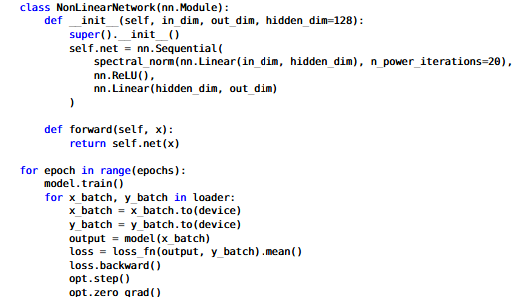
\includegraphics[width=0.8\linewidth]{BilderPräsentation/TrainNN.png}
%	\end{figure}
%\end{frame}
%\endgroup 

\begingroup
\frametitle{Reproduktion der Intrinsic Homotopy Werte}
\begin{frame}{Reproduktion der Intrinsic Homotopy Werte}
	\begin{columns}
	\column{0.4\textwidth}
	\begin{minipage}[t]{\linewidth}
		\vspace{1em}
		\begin{itemize}
			\tiny
			\uncover<1->{\item  Ziel: Reproduktion der Distanzwerte aus Chan et al.~\cite{chan_affine_2024}}
			\uncover<2->{\item Erster Versuch: Approximation der Werte im Testsplit, selber Architektur und $\max(\text{loss})$}
			\uncover<3->{\item Zweiter Versuch: Approximation der Werte mit im Trainingssplit, selber Architektur und $\max(\text{loss})$}
			\uncover<4->{\item Modelle sind aufgrund des Trainings auf den Trainingsdaten gebiased, daher erfolgen Tests auf einem separaten Testsplit}
		\end{itemize}
	\end{minipage}
	\column{0.6\textwidth}
\uncover<1->{	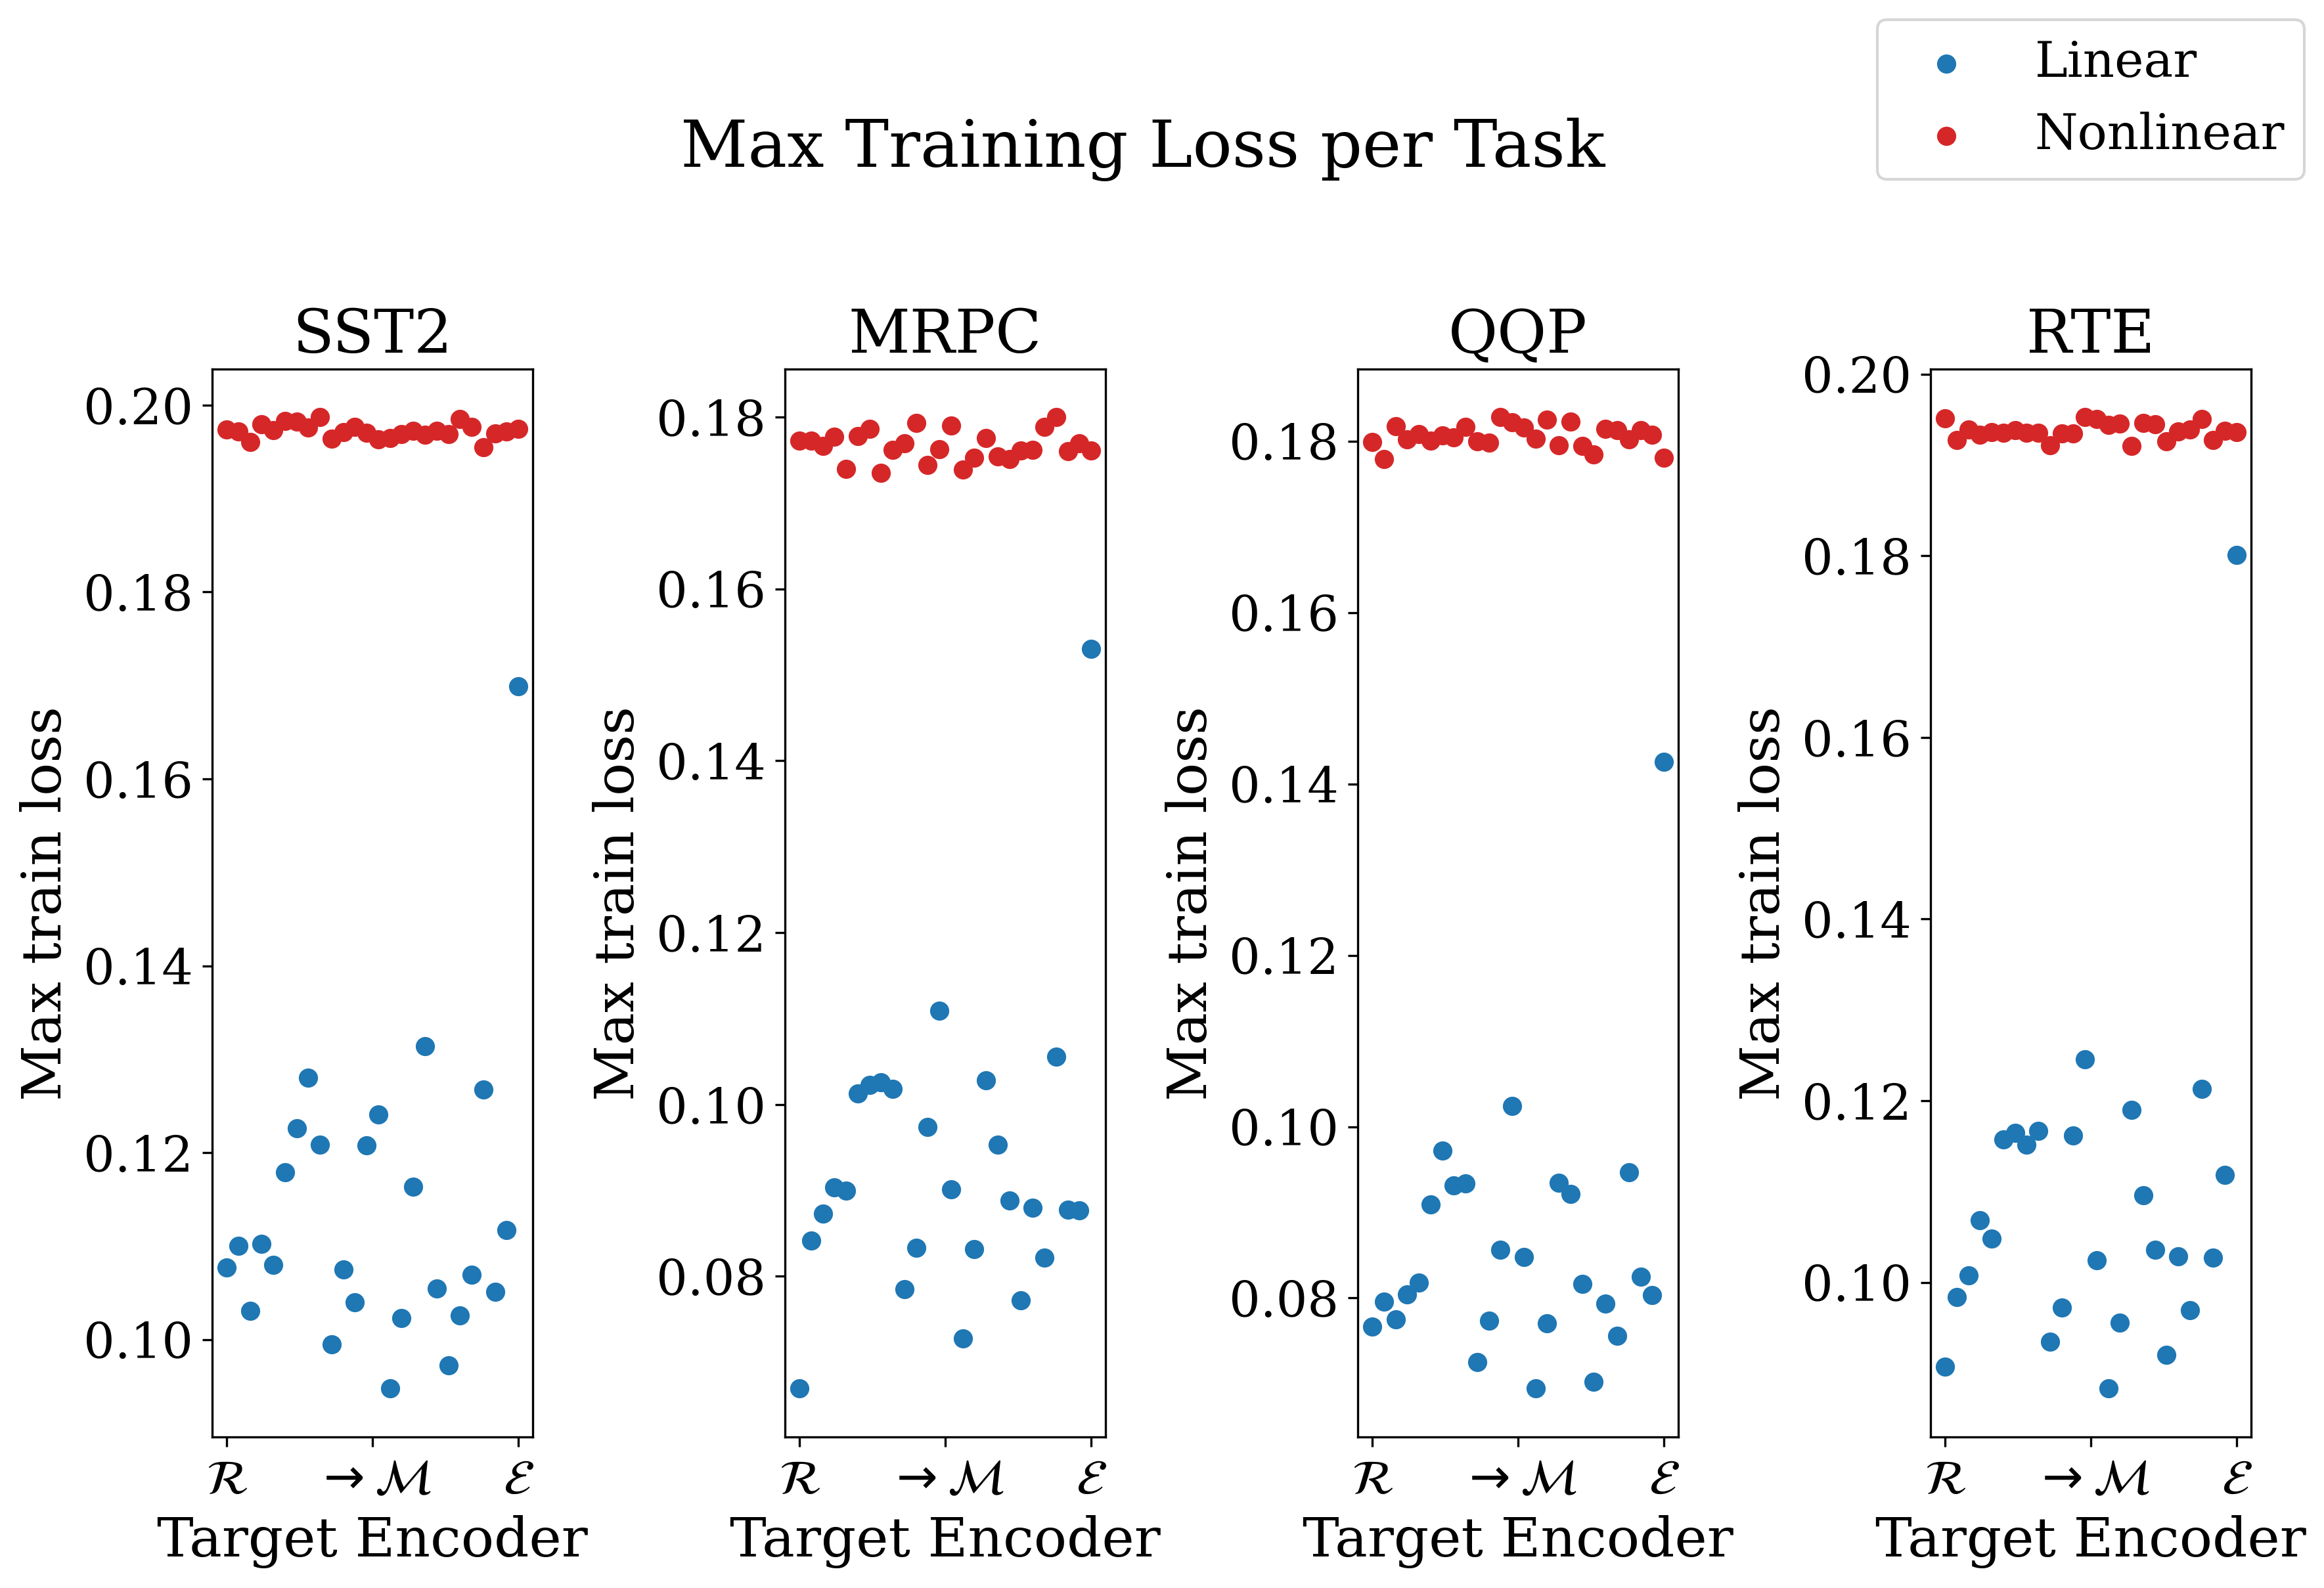
\includegraphics[width=\linewidth]{BilderPräsentation/New_all_in_one_scatter_praes.png}}
\end{columns}
\end{frame}
\endgroup


\begingroup
\frametitle{Experiment: Intrinsic Homotopy}
\begin{frame}
	\begin{columns}
		\column{0.4\textwidth}
		\begin{minipage}[t]{\linewidth}
			\vspace{1em}
			\tiny
			\begin{itemize}
				\tiny
				\uncover<1->{\item Analyse linearer und nicht-linearer Transformationen}
			\end{itemize}
		\end{minipage}
		
		\column{0.6\textwidth}
		\uncover<2->{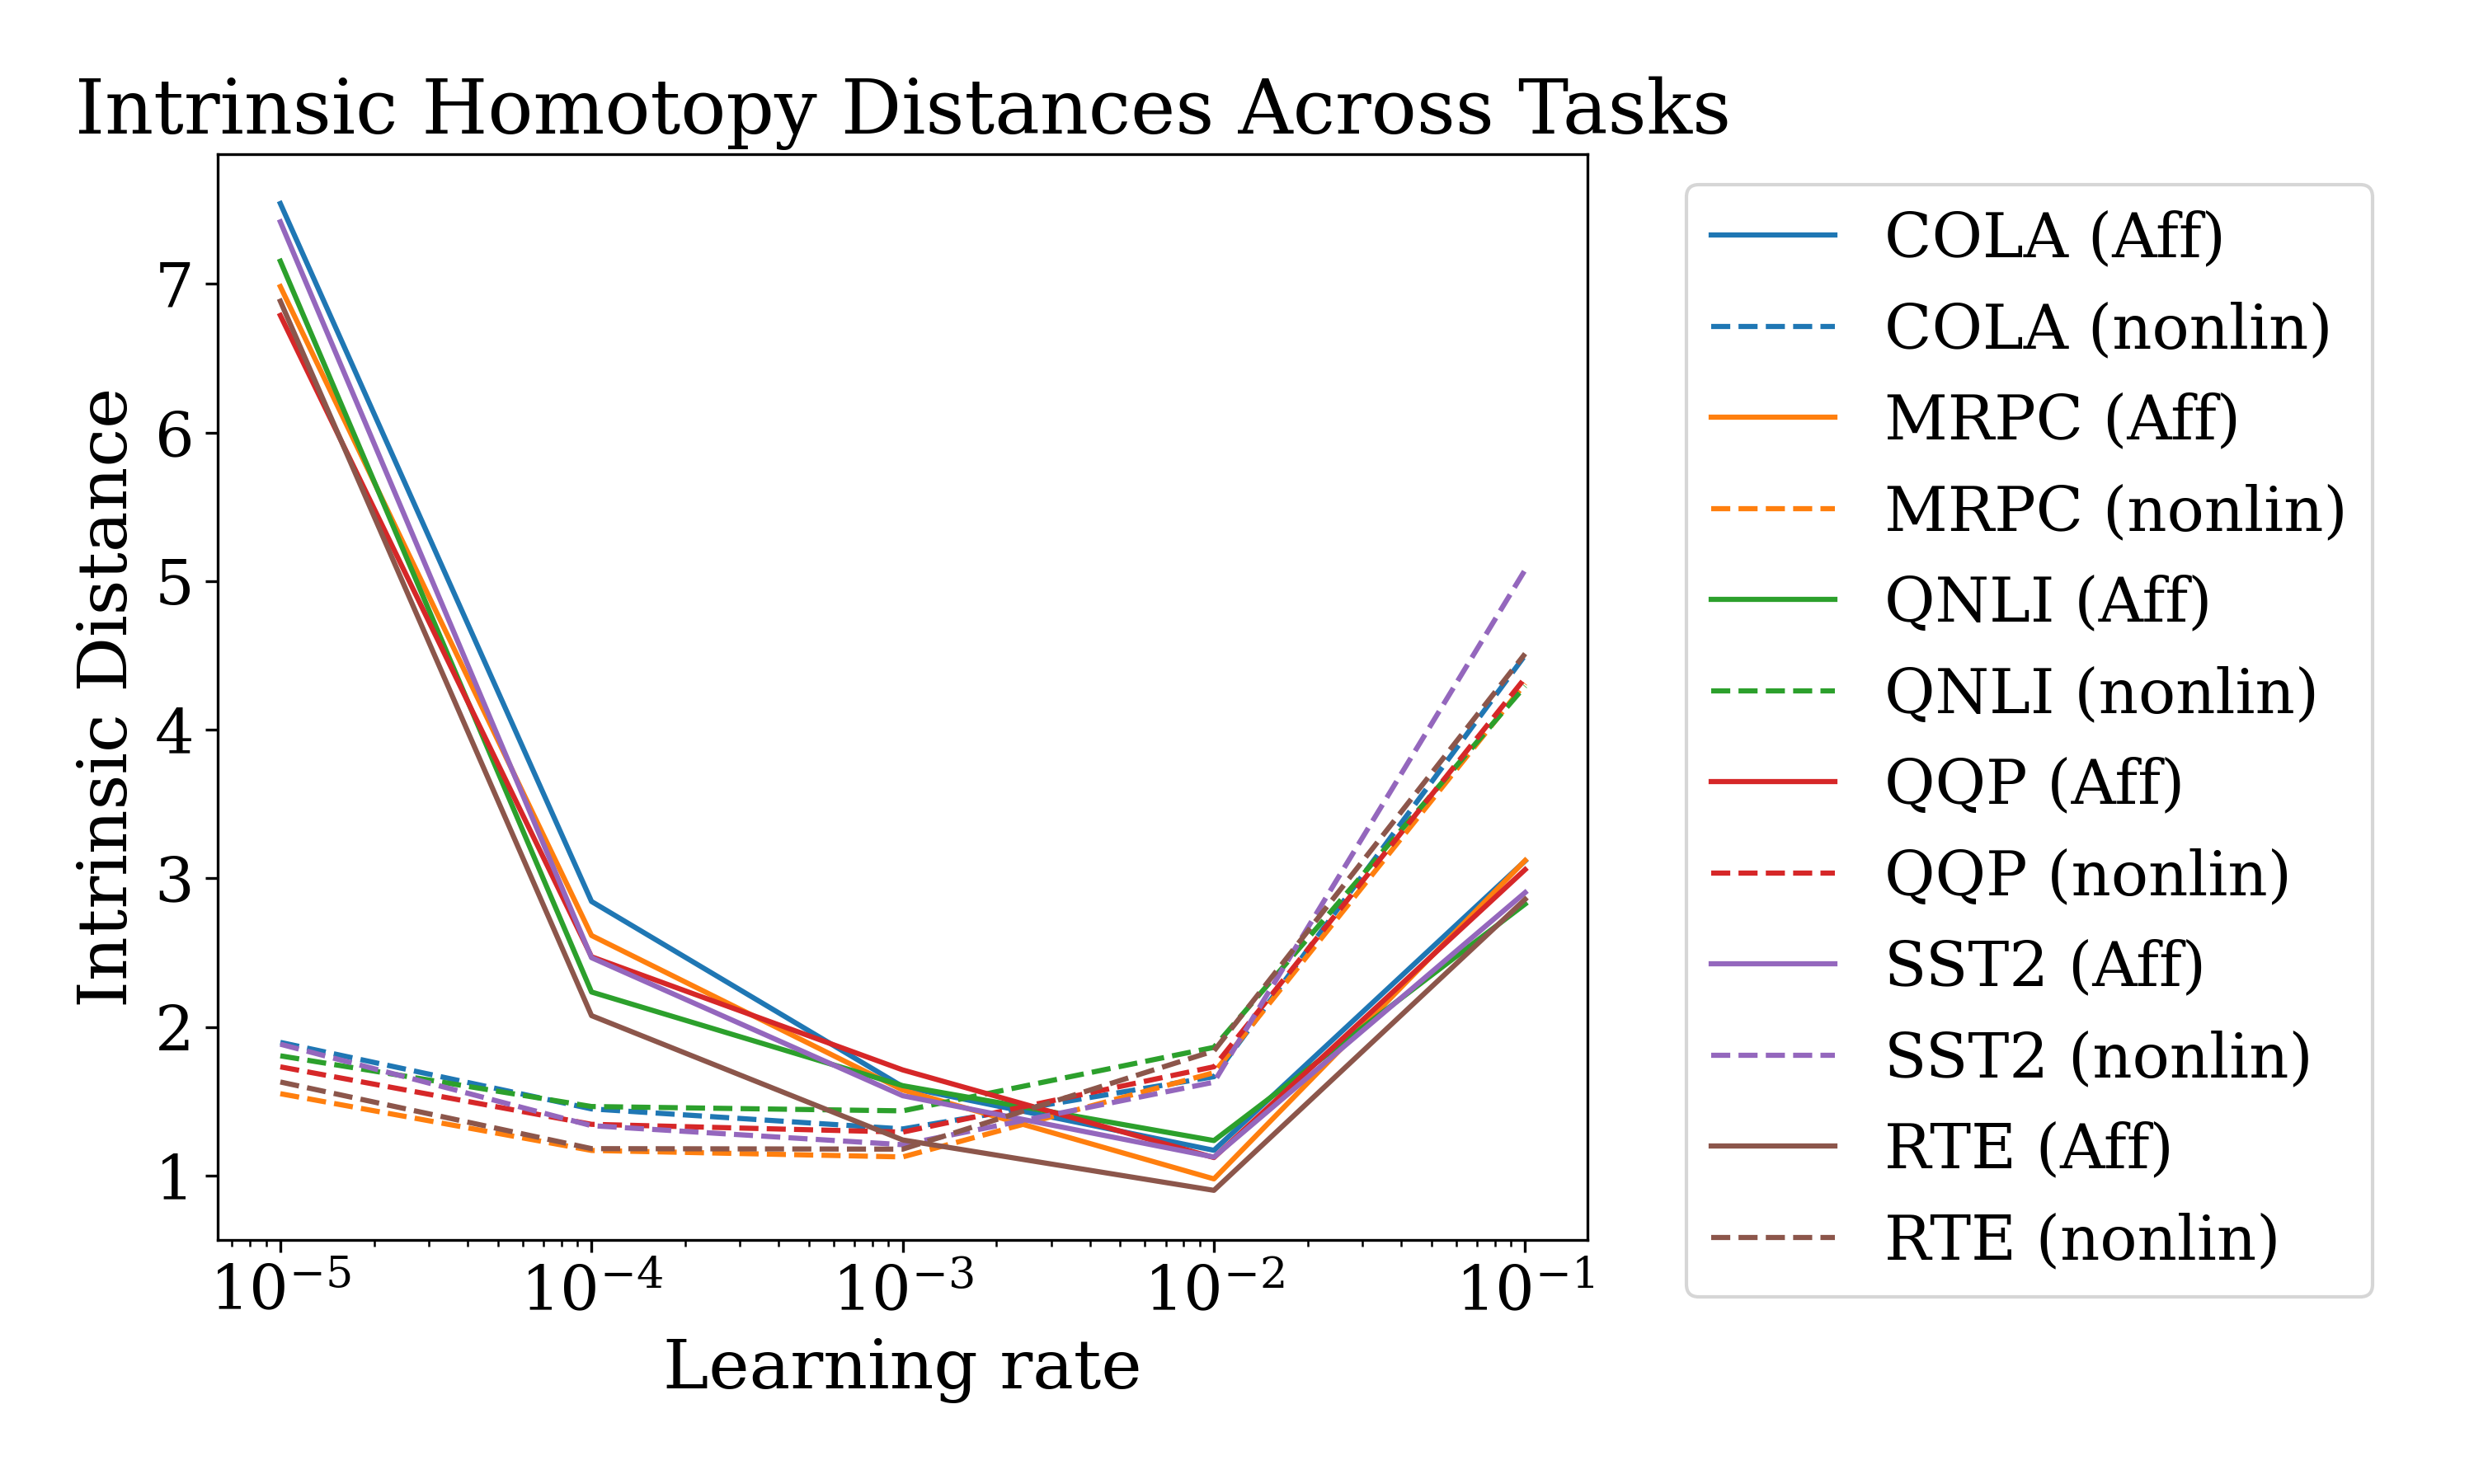
\includegraphics[width=1.1\linewidth]{BilderPräsentation/intrinsic_distance_all_tasksPräsi.png}}
	\end{columns}
\end{frame}
\endgroup

\begingroup
\frametitle{Experiment: Intrinsic Homotopy}
\begin{frame}
			\vspace{1em}
			\tiny
			\begin{itemize}
				\tiny
				\uncover<1->{\item Analyse linearer und nicht-linearer Transformationen}
				\uncover<2->{\item Pearson-Koeffizient: zeigt linearen Zusammenhang zwischen Input und Output}
				\uncover<3->{\item Kaum linearer Zusammenhang $\Longrightarrow$ schwierig, lineare Transformation zu finden}
				\uncover<4->{\item Lineare Modelle reichen nicht aus, um Strukturähnlichkeit realistisch abzubilden}
			\end{itemize}
		\begin{table}[H]
			\centering
			\caption{Pearson Correlation Score \(r\) across tasks and learning rates.}
			\label{tab:correlation-transposed}
			\begin{tabular}{l c ccccccc}
				\toprule
				 & \texttt{QNLI} & \texttt{CoLA} & \texttt{MRPC} & \texttt{QQP} & \texttt{RTE} & \texttt{SST-2} \\
				\midrule
				\(r\) 
				&  \(5\cdot10^{-6}\) & \(4\cdot10^{-6}\) & \(4\cdot10^{-6}\) & \(5\cdot10^{-6}\) & \(3\cdot10^{-6}\) & \(5\cdot10^{-6}\)
			\end{tabular}
		\end{table}
\end{frame}
\endgroup




\begingroup
\frametitle{Experiment: Intrinsic Homotopy}
\begin{frame}
	\begin{columns}
		\column{0.4\textwidth}
		\begin{minipage}[t]{\linewidth}
			\vspace{1em}
			\tiny
			\begin{itemize}
				\tiny
				\uncover<1->{\item \textbf{Beispiel-Task:} \textbf{MRPC} – geringste Distanzen im Intrinsic-Vergleich}
				\uncover<2->{\item \textbf{Heatmaps:} Modelle mit $d_{\mathcal{C}}(h, g) < 1$  und  $d_{\mathcal{C}}(g, h) < 1$ gelten als \emph{homotop} (weiß markiert)}
				\uncover<3->{\item \textbf{Beobachtungen:}}
				\begin{itemize}
					\tiny
					\uncover<4->{\item Deutlich mehr homotope Modellpaare bei \textbf{nichtlinearen Transformationen}}
					\uncover<5->{\item Besonders bei kleinen Lernraten (\texttt{lr} = $10^{-5}$ bis $10^{-3}$)}
					\uncover<6->{\item Höhere Lernraten $\Rightarrow$ instabileres Training, weniger Struktur}
				\end{itemize}
			\end{itemize}
		\end{minipage}
		
		\column{0.6\textwidth}
		\uncover<2->{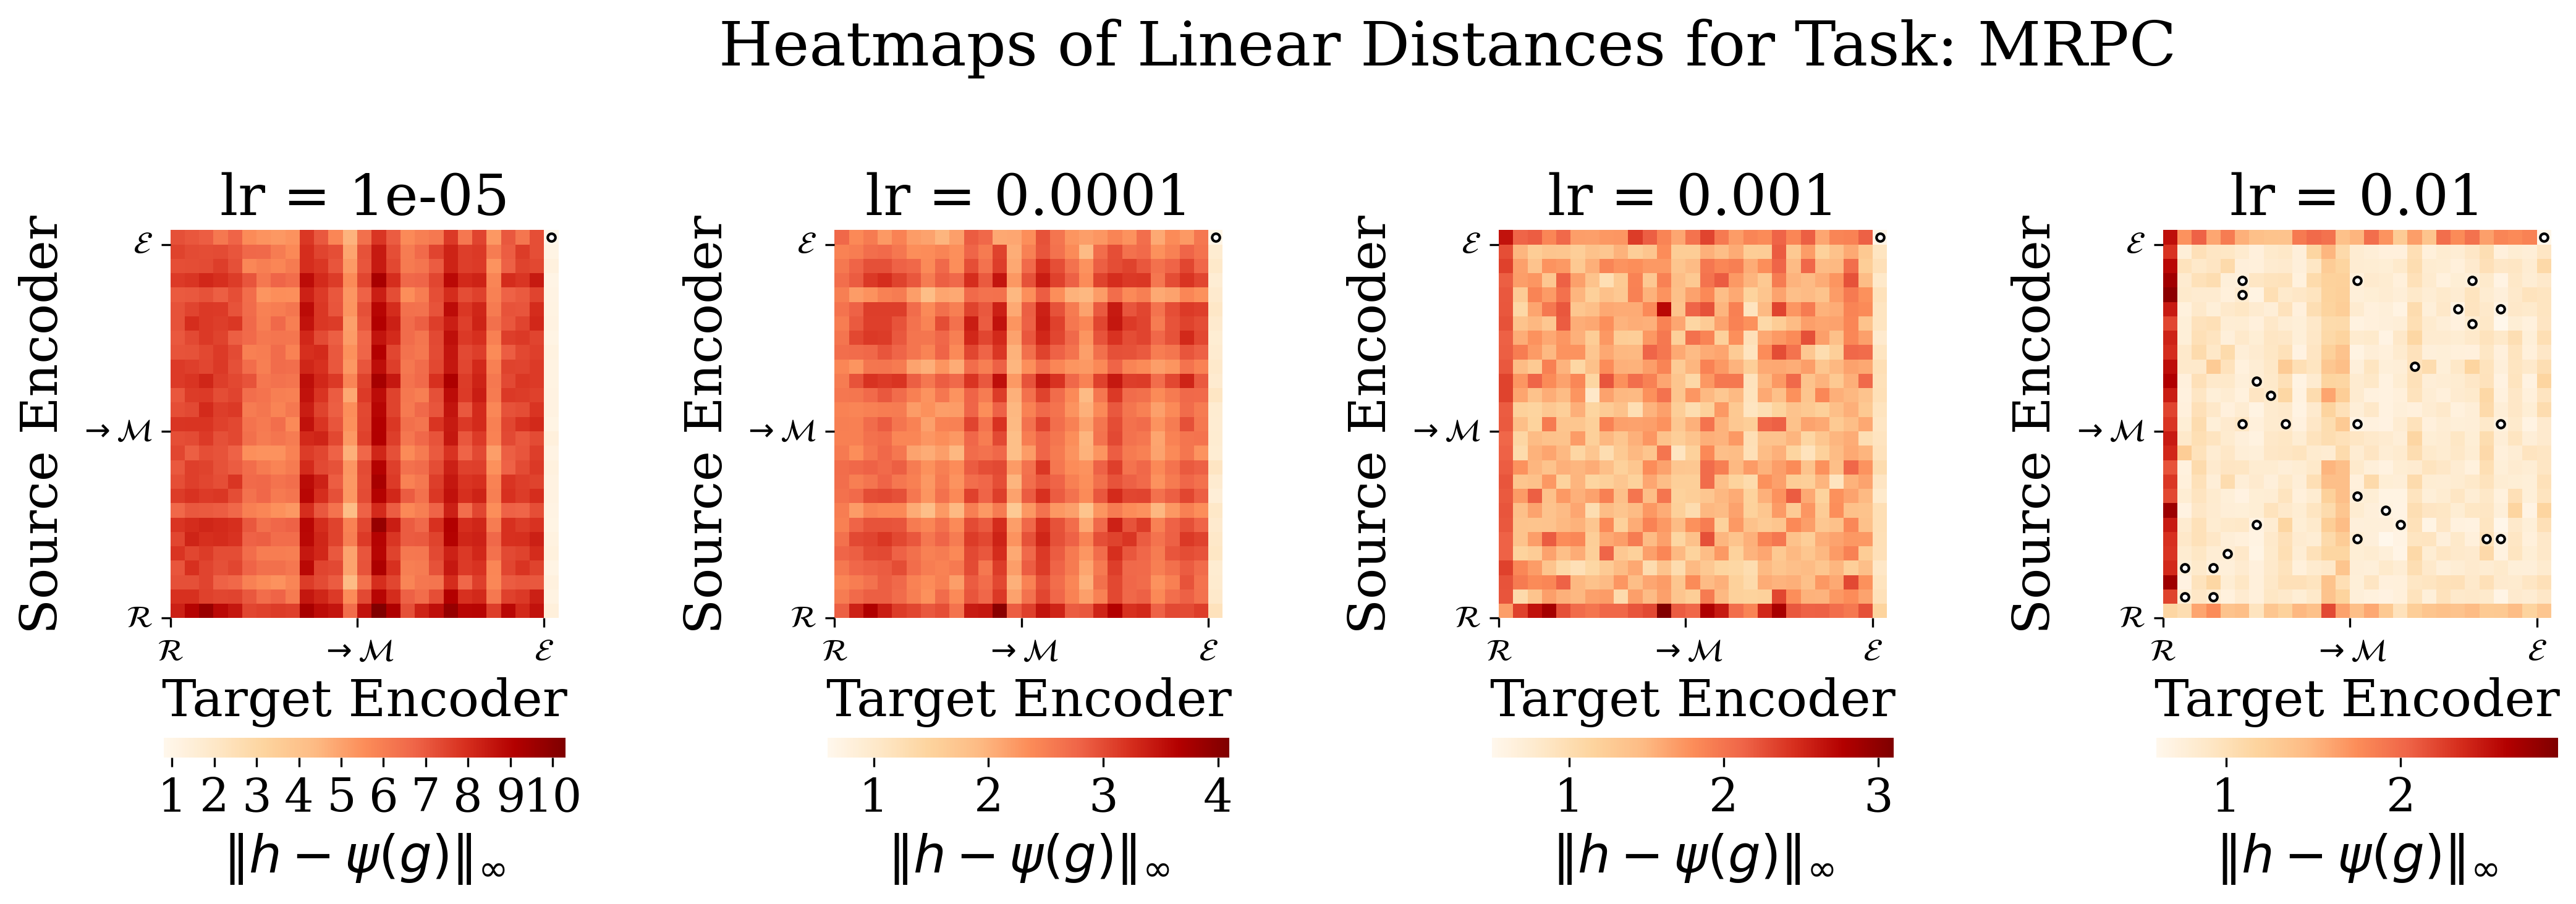
\includegraphics[width=\linewidth]{BilderPräsentation/PräsiHeatmap_linear_distance_all_lrs_mrpc_homotopy.png}\\[1ex]}
		\uncover<2->{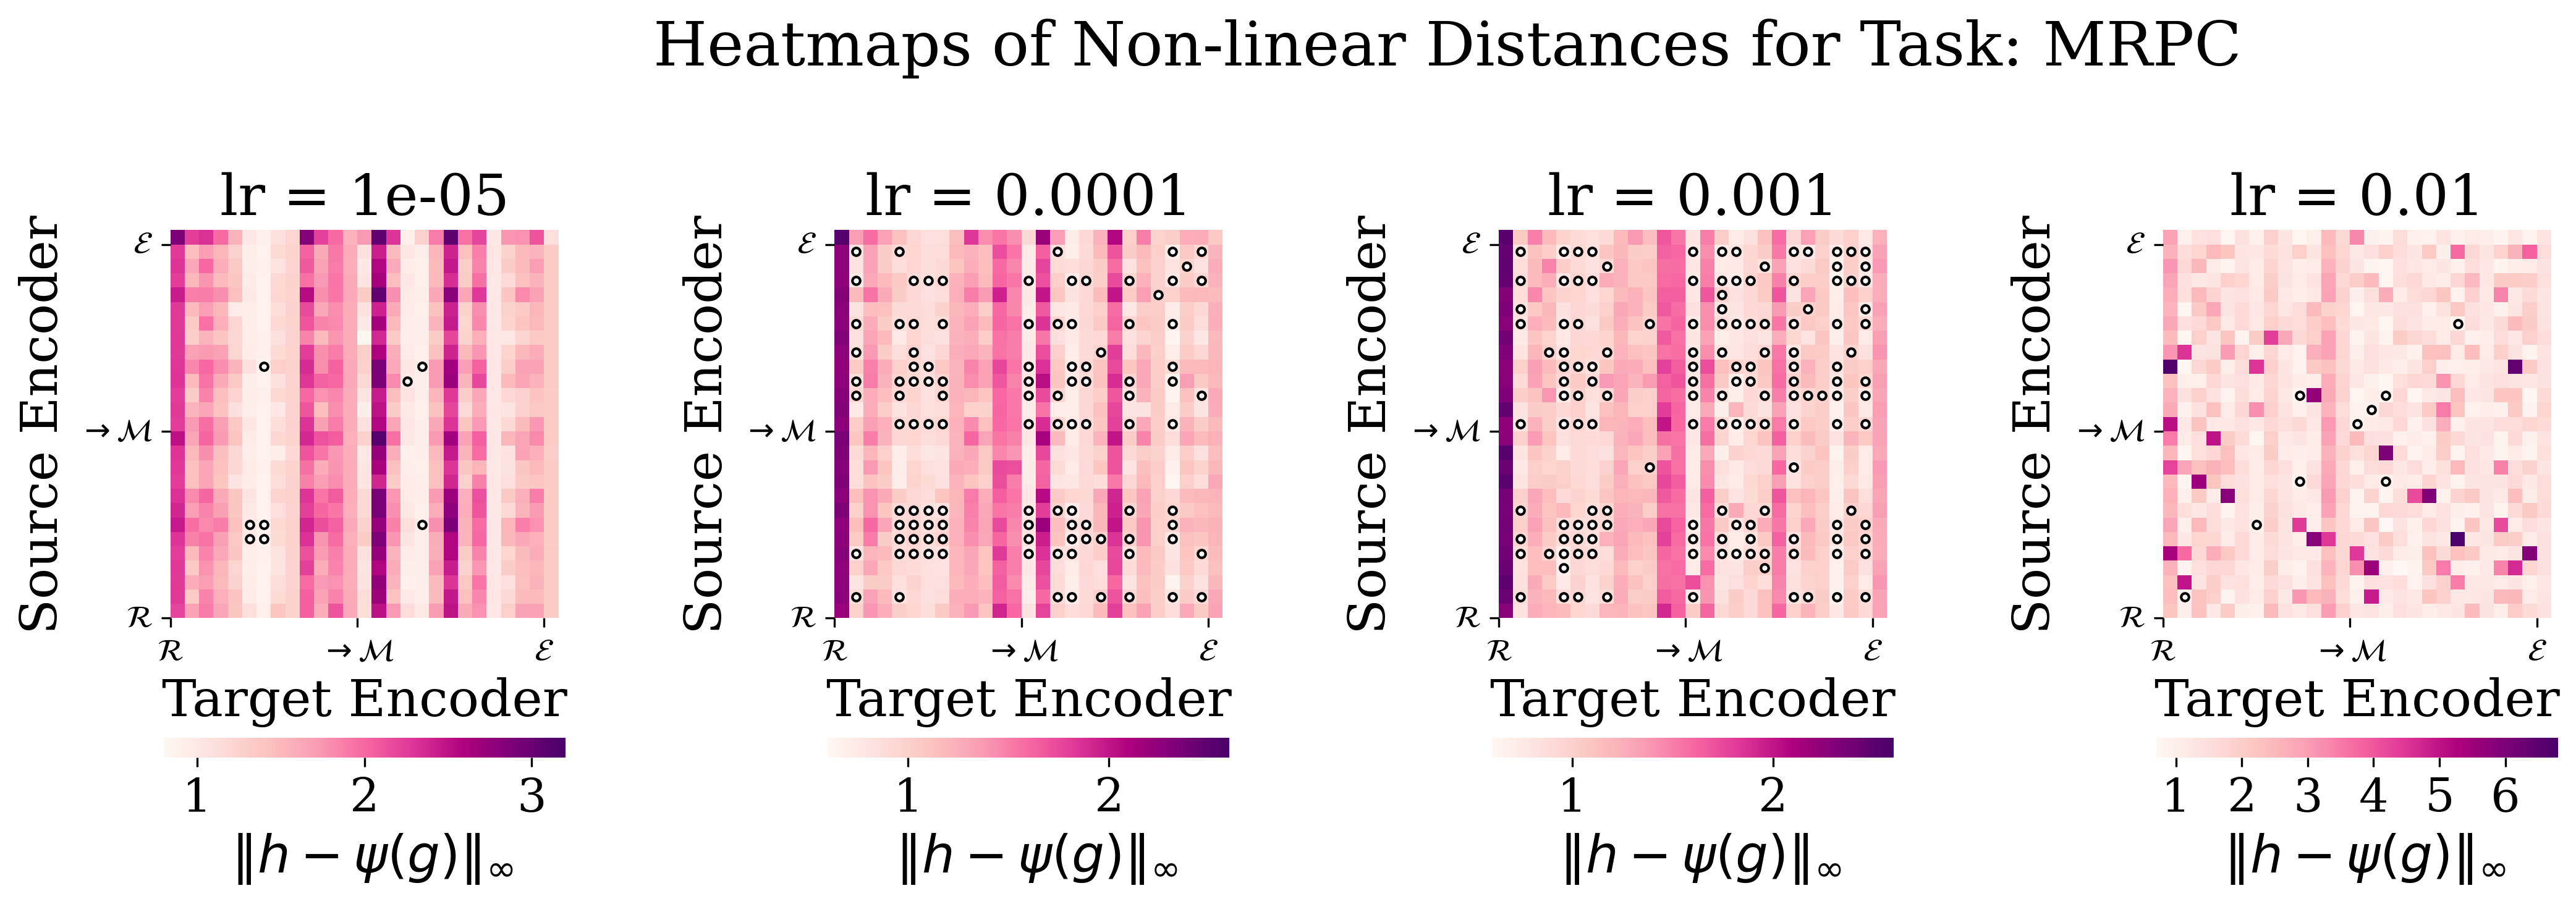
\includegraphics[width=\linewidth]{BilderPräsentation/PräsiHeatmap_nonlinear_distance_all_lrs_mrpc_homotopy.png}}
	\end{columns}
\end{frame}
\endgroup


\begingroup
\frametitle{Experiment: Intrinsic vs Extrinsic Homotopy}
\begin{frame}
	\tiny
	\begin{itemize}
		\tiny
		\uncover<1->{\item Intrinsic $\Rightarrow$ Extrinsic in Chan et al.~\cite{chan_affine_2024}} 
		\uncover<2->{\item \textbf{Beobachtungen:}}
		\begin{itemize}
			\tiny
			\uncover<2->{\item Beste Übereinstimmung bei \textbf{QNLI} (höchste Regressionsgüte)}
			\uncover<2->{\item Aber selbst hier nur leichter zusammenhang }
		\end{itemize}
	\end{itemize}
	\vspace{1em}
	\uncover<2->{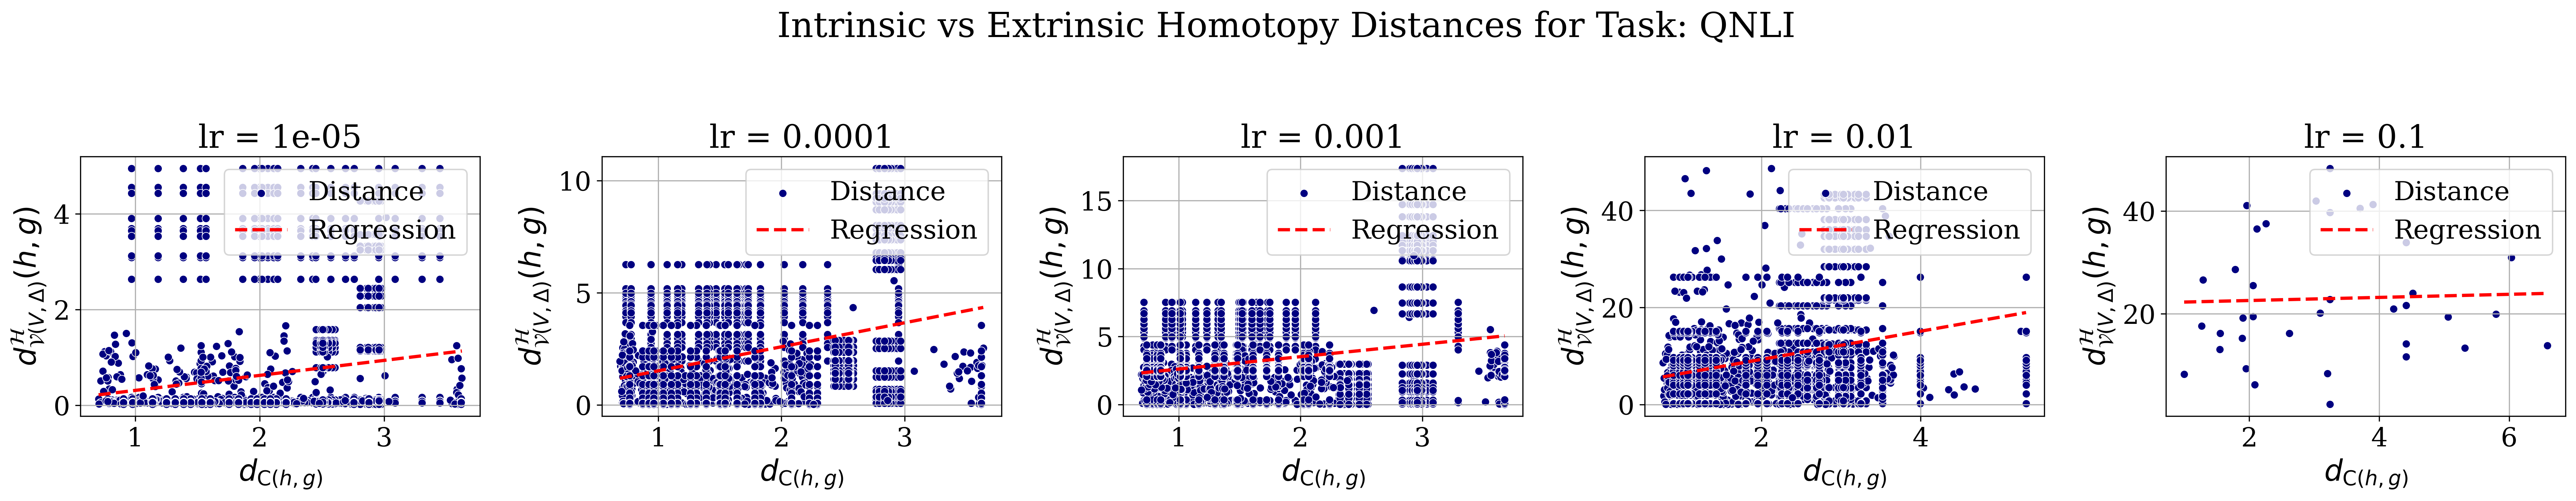
\includegraphics[width=1\linewidth]{BilderPräsentation/intrinsicVSextrinsic/PräsiDist_extr_intr_subplots_qnli.png}}
\end{frame}
\endgroup

\begingroup
\frametitle{Experiment: Intrinsic vs Extrinsic Homotopy}
\begin{frame}
	\tiny
	\begin{itemize}
		\tiny
		\uncover<1->{\item \textbf{Beobachtungen:}}
		\begin{itemize}
			\tiny
			\uncover<1->{\item Regressionslinie bei \textbf{MRPC} nahezu parallel zur X-Achse }
			\uncover<1->{\item $\Rightarrow$ Kaum Zusammenhang zwischen intrinsischer und extrinsischer Ähnlichkeit in unserem Setup, stark vom Task abhängig}
		\end{itemize}
	\end{itemize}
	\vspace{1em}
		\uncover<1->{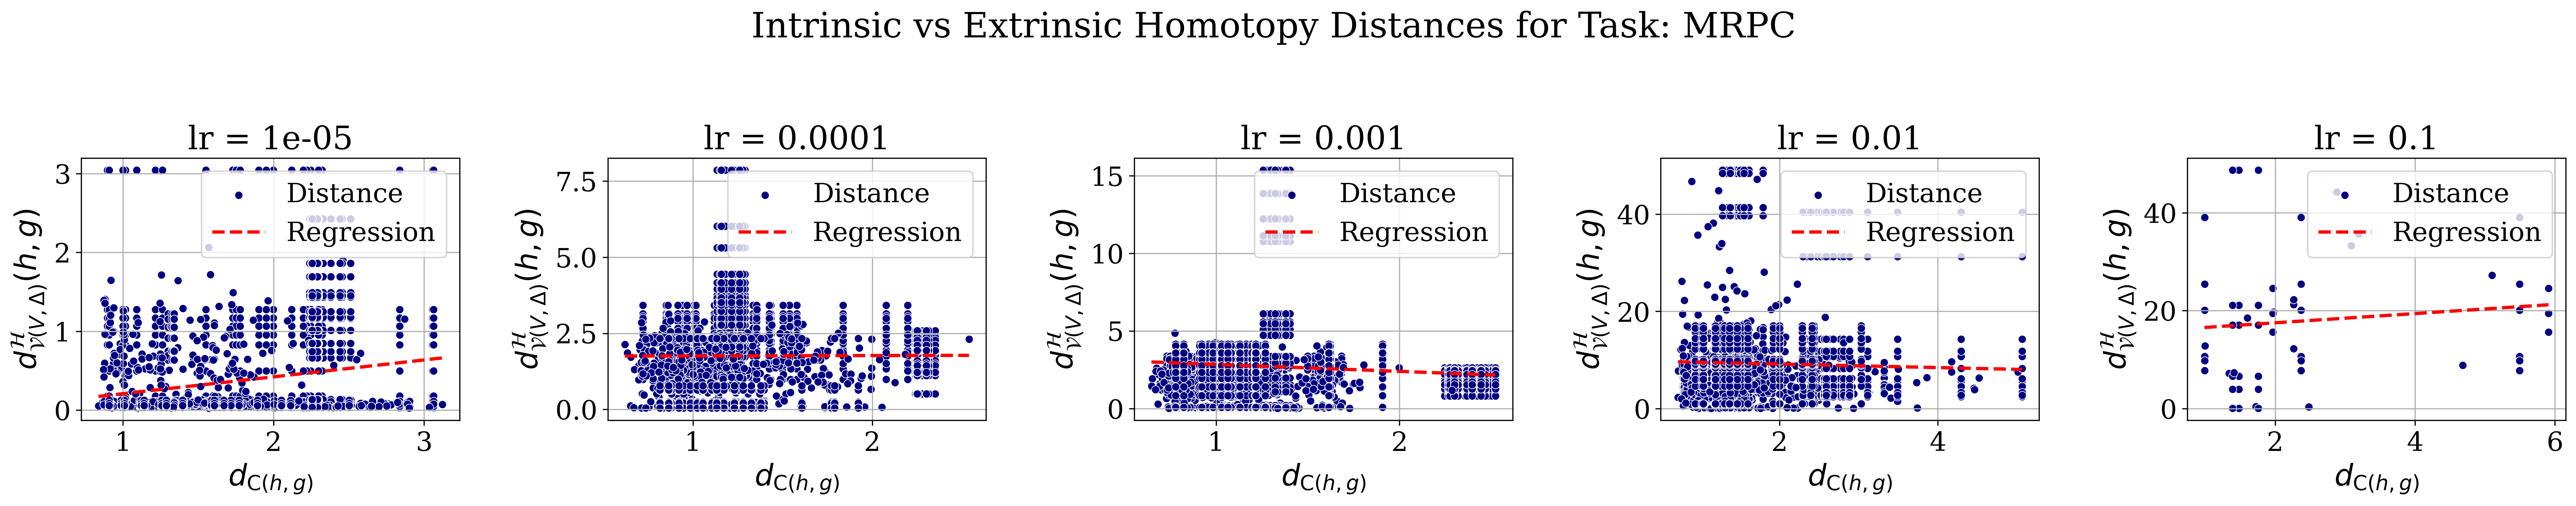
\includegraphics[width=1\linewidth]{BilderPräsentation/intrinsicVSextrinsic/PräsiDist_extr_intr_subplots_mrpc.png}}
\end{frame}
\endgroup

